\subsection{Métricas de Evaluación para Sistemas de Clasificación}

La evaluación cuantitativa del desempeño de sistemas de clasificación requiere métricas robustas que capturen diferentes aspectos de la calidad predictiva. En aplicaciones de agricultura de precisión, donde decisiones incorrectas pueden impactar la productividad del cultivo, resulta fundamental comprender las fortalezas y limitaciones de cada métrica.

\subsubsection{Matriz de Confusión}

La matriz de confusión constituye la representación fundamental del desempeño de un clasificador, tabulando predicciones versus etiquetas verdaderas. Para un problema de $C$ clases, la matriz de confusión $\mathbf{M} \in \mathbb{R}^{C \times C}$ se define como:

\begin{equation}
M_{ij} = \sum_{k=1}^{N} \mathbb{1}[y_k = i \land \hat{y}_k = j]
\end{equation}

donde $y_k$ es la clase verdadera de la muestra $k$, $\hat{y}_k$ es la clase predicha, y $\mathbb{1}[\cdot]$ es la función indicadora.

Para clasificación binaria, la matriz se simplifica a:

\begin{equation}
\mathbf{M} = \begin{bmatrix}
\text{TN} & \text{FP} \\
\text{FN} & \text{TP}
\end{bmatrix}
\end{equation}

donde:
\begin{itemize}
\item \textbf{TP (True Positives)}: Casos positivos correctamente clasificados
\item \textbf{TN (True Negatives)}: Casos negativos correctamente clasificados  
\item \textbf{FP (False Positives)}: Casos negativos incorrectamente clasificados como positivos (Error Tipo I)
\item \textbf{FN (False Negatives)}: Casos positivos incorrectamente clasificados como negativos (Error Tipo II)
\end{itemize}

\begin{figure}[h]
\centering
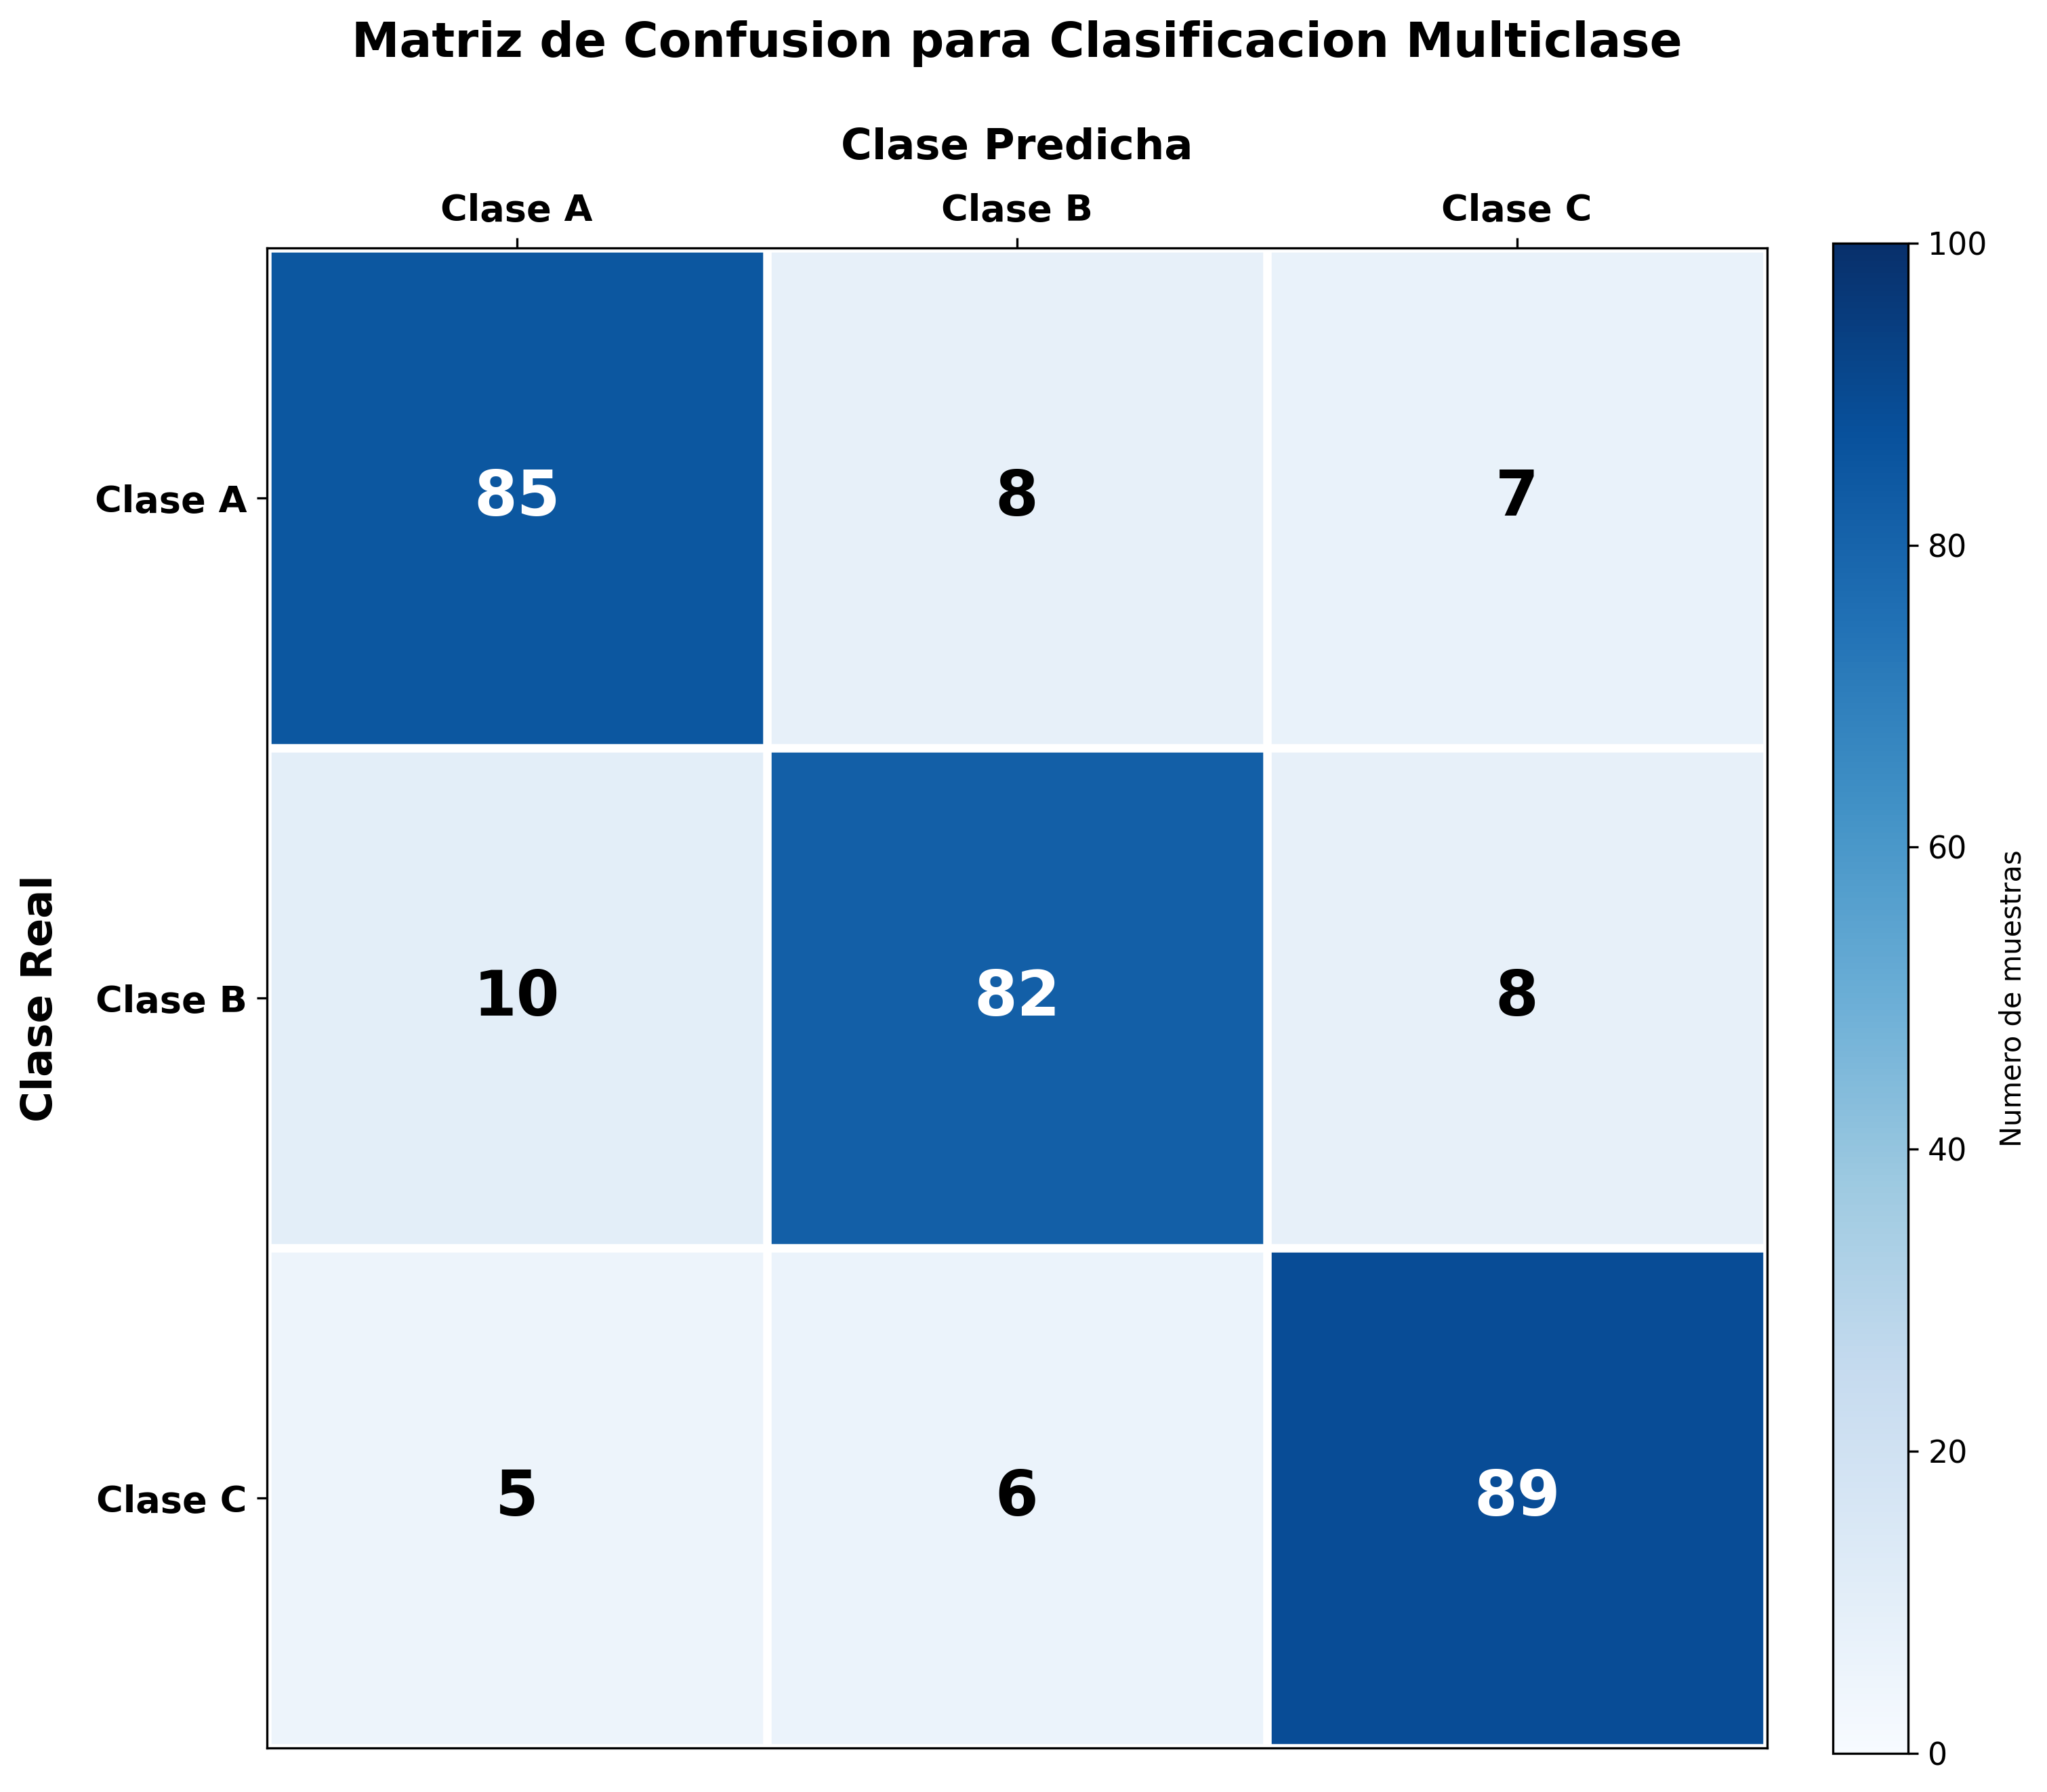
\includegraphics[width=0.6\textwidth]{imagenes/matriz_confusion_ejemplo.png}
\caption{Matriz de confusión para clasificación multiclase mostrando patrones de error}
\label{fig:matriz_confusion}
\end{figure}

\subsubsection{Exactitud (Accuracy)}

La exactitud mide la proporción global de predicciones correctas:

\begin{equation}
\text{Accuracy} = \frac{\text{TP} + \text{TN}}{\text{TP} + \text{TN} + \text{FP} + \text{FN}} = \frac{\sum_{i=1}^{C} M_{ii}}{N}
\end{equation}

\textbf{Ventajas:}
\begin{itemize}
\item Interpretación intuitiva: porcentaje de aciertos
\item Métrica estándar para comparación entre modelos
\item Apropiada cuando todas las clases tienen igual importancia
\end{itemize}

\textbf{Limitaciones Críticas}

La exactitud resulta engañosa en datasets desbalanceados. Considere un clasificador que siempre predice la clase mayoritaria en un dataset con 95\% de negativos:

\begin{equation}
\text{Accuracy}_{naive} = \frac{0.95N}{N} = 0.95
\end{equation}

Este clasificador trivial alcanza 95\% de exactitud sin aprender ningún patrón útil. En agricultura, donde ciertas condiciones pueden ser raras pero críticas, la exactitud puede ocultar fallos graves del modelo.

\subsubsection{Precisión (Precision)}

La precisión cuantifica la proporción de predicciones positivas que son correctas:

\begin{equation}
\text{Precision} = \frac{\text{TP}}{\text{TP} + \text{FP}}
\end{equation}

\textbf{Interpretación:} De todas las instancias que el modelo clasificó como positivas, ¿qué fracción realmente lo era?

Para clasificación multiclase, se calcula precisión por clase:

\begin{equation}
\text{Precision}_i = \frac{M_{ii}}{\sum_{j=1}^{C} M_{ji}}
\end{equation}

La precisión es crucial cuando el costo de falsos positivos es alto. En cosecha automatizada, alta precisión garantiza que el robot no intente cosechar elementos no deseados.

\subsubsection{Exhaustividad (Recall/Sensitivity)}

El recall mide la proporción de casos positivos reales que fueron correctamente identificados:

\begin{equation}
\text{Recall} = \frac{\text{TP}}{\text{TP} + \text{FN}}
\end{equation}

\textbf{Interpretación:} De todas las instancias que realmente son positivas, ¿qué fracción detectó el modelo?

Para clasificación multiclase:

\begin{equation}
\text{Recall}_i = \frac{M_{ii}}{\sum_{j=1}^{C} M_{ij}}
\end{equation}

El recall es fundamental cuando el costo de falsos negativos es alto. En detección de elementos para cosecha, alto recall asegura que no se pierdan productos maduros.

\subsubsection{F-Score}

El F-Score armoniza precisión y recall mediante su media armónica:

\begin{equation}
F_1 = 2 \cdot \frac{\text{Precision} \cdot \text{Recall}}{\text{Precision} + \text{Recall}} = \frac{2\text{TP}}{2\text{TP} + \text{FP} + \text{FN}}
\end{equation}

\textbf{Generalización F-Beta}

Cuando se desea ponderar diferentemente precisión y recall:

\begin{equation}
F_\beta = (1 + \beta^2) \cdot \frac{\text{Precision} \cdot \text{Recall}}{\beta^2 \cdot \text{Precision} + \text{Recall}}
\end{equation}

\begin{itemize}
\item $\beta < 1$: Favorece precisión
\item $\beta = 1$: Balance equitativo (F1-Score)
\item $\beta > 1$: Favorece recall
\end{itemize}

\begin{figure}[h]
\centering
\includegraphics[width=0.7\textwidth]{imagenes/tradeoff_precision_recall.png}
\caption{Trade-off entre precisión y recall para diferentes valores de umbral}
\label{fig:tradeoff}
\end{figure}

\subsubsection{Métricas Agregadas Multiclase}

Para problemas con $C > 2$ clases, las métricas por clase se agregan mediante:

\textbf{Macro-Average}

Promedio simple de métricas por clase:

\begin{equation}
\text{Metric}_{macro} = \frac{1}{C}\sum_{i=1}^{C} \text{Metric}_i
\end{equation}

Trata todas las clases por igual, apropiado cuando cada clase tiene igual importancia independientemente de su frecuencia.

\textbf{Weighted-Average}

Promedio ponderado por soporte de cada clase:

\begin{equation}
\text{Metric}_{weighted} = \frac{1}{N}\sum_{i=1}^{C} n_i \cdot \text{Metric}_i
\end{equation}

donde $n_i = \sum_{j=1}^{C} M_{ij}$ es el número de instancias verdaderas de clase $i$.

\textbf{Micro-Average}

Calcula métricas globales agregando TP, FP, FN de todas las clases:

\begin{equation}
\text{Precision}_{micro} = \frac{\sum_{i=1}^{C} \text{TP}_i}{\sum_{i=1}^{C} (\text{TP}_i + \text{FP}_i)}
\end{equation}

\subsubsection{Métricas de Error Absoluto}

Para clasificadores basados en descriptores continuos, es relevante evaluar el error en la estimación del descriptor mismo.

\textbf{Error Absoluto Medio (MAE)}

\begin{equation}
\text{MAE} = \frac{1}{N}\sum_{i=1}^{N}|y_i - \hat{y}_i|
\end{equation}

Mide la magnitud promedio de los errores sin considerar su dirección.

\textbf{Error Cuadrático Medio (RMSE)}

\begin{equation}
\text{RMSE} = \sqrt{\frac{1}{N}\sum_{i=1}^{N}(y_i - \hat{y}_i)^2}
\end{equation}

Penaliza errores grandes más fuertemente que MAE debido a la elevación al cuadrado.

\textbf{Error Porcentual Absoluto Medio (MAPE)}

\begin{equation}
\text{MAPE} = \frac{100\%}{N}\sum_{i=1}^{N}\left|\frac{y_i - \hat{y}_i}{y_i}\right|
\end{equation}

Expresa el error como porcentaje del valor verdadero, útil para comparar desempeño en magnitudes diferentes.

\begin{figure}[h]
\centering
\includegraphics[width=0.7\textwidth]{imagenes/distribucion_errores.png}
\caption{Distribución de errores absolutos en la estimación de descriptores}
\label{fig:errores}
\end{figure}

\subsubsection{Coeficiente de Determinación}

Para regresión de descriptores continuos, el coeficiente $R^2$ mide la proporción de varianza explicada:

\begin{equation}
R^2 = 1 - \frac{\sum_{i=1}^{N}(y_i - \hat{y}_i)^2}{\sum_{i=1}^{N}(y_i - \bar{y})^2}
\end{equation}

donde $\bar{y}$ es la media de los valores observados.

\textbf{Interpretación:}
\begin{itemize}
\item $R^2 = 1$: Predicción perfecta
\item $R^2 = 0$: Modelo no mejor que predecir la media
\item $R^2 < 0$: Modelo peor que predecir la media
\end{itemize}

\subsubsection{Métricas de Confiabilidad}

\textbf{Intervalo de Confianza}

Para una métrica estimada $\hat{\theta}$ con error estándar $SE$, el intervalo de confianza al $(1-\alpha)100\%$ es:

\begin{equation}
\text{IC}_{1-\alpha} = \hat{\theta} \pm z_{\alpha/2} \cdot SE
\end{equation}

Para exactitud:

\begin{equation}
SE_{Acc} = \sqrt{\frac{\hat{p}(1-\hat{p})}{n}}
\end{equation}

\textbf{Coeficiente de Variación}

Mide la variabilidad relativa de una métrica:

\begin{equation}
CV = \frac{\sigma}{\mu} \times 100\%
\end{equation}

Valores bajos de CV indican consistencia del clasificador entre diferentes conjuntos de prueba.

\subsubsection{Métricas de Robustez}

\textbf{Estabilidad ante Perturbaciones}

Evalúa degradación de desempeño bajo ruido:

\begin{equation}
\Delta\text{Perf} = \frac{\text{Perf}_{clean} - \text{Perf}_{noisy}}{\text{Perf}_{clean}} \times 100\%
\end{equation}

Sistemas robustos exhiben $\Delta\text{Perf} < 10\%$ para niveles moderados de ruido.

\textbf{Repetibilidad}

Desviación estándar de la métrica en ejecuciones repetidas:

\begin{equation}
\sigma_{rep} = \sqrt{\frac{1}{K-1}\sum_{k=1}^{K}(\text{Metric}_k - \bar{\text{Metric}})^2}
\end{equation}

donde $K$ es el número de repeticiones.

\begin{figure}[h]
\centering
\includegraphics[width=0.7\textwidth]{imagenes/robustez_ruido.png}
\caption{Degradación de exactitud con incremento de ruido gaussiano}
\label{fig:robustez}
\end{figure}

\subsubsection{Selección de Métricas según Aplicación}

Para sistemas de clasificación en agricultura de precisión, la selección de métricas debe alinearse con los objetivos operativos:

\textbf{Prioridades Típicas:}
\begin{enumerate}
\item \textbf{Alta Exhaustividad}: Minimizar productos no detectados
\item \textbf{Precisión Aceptable}: Limitar clasificaciones incorrectas
\item \textbf{Robustez}: Mantener desempeño bajo variaciones ambientales
\item \textbf{Consistencia}: Bajo coeficiente de variación entre sesiones
\end{enumerate}

La métrica compuesta óptima puede definirse como:

\begin{equation}
\text{Score}_{total} = w_1 \cdot F_\beta + w_2 \cdot (1 - CV) + w_3 \cdot (1 - \Delta\text{Perf})
\end{equation}

donde $w_i$ son pesos que reflejan la importancia relativa de cada aspecto, con $\sum w_i = 1$.